\chapter{Auswertung}
Die Ergebnisse zur Gesamtbewertung finden sich in Tabelle \ref{tab:Auswertung}. Diese beinhaltet die Hardware, welche zum Großteil durch die Induktivitäten beeinflusst wird, sowie die Kapazitäten, Halbleiter und Treiber. Außerdem werden die Ergebnisse der Simulation durch die Verlustleistung der Halbleiter bewertet. Für die Simulation werden die in Tabelle \ref{tab:Betriebspara} aufgelisteten Betriebsparameter festgelegt. Die beiden Topologien werden für den Betriebspunkt mit 0° und 30° Phasenverschiebung verglichen, um den Einfluss der Systemdienstleistungen zu betrachten. Um einen Vergleich der Kategorien und eine Gesamtbewertung durchzuführen, werden die Einzelkategorien zwischen null und eins normiert und mit einem Gewichtungsfaktor die Summe über alle Kategorien gebildet. Aufgrund des großen Einflusses der Drosseln, werden diese mit 50 Prozent gewichtet. Die Kapazitäten stellen nur einen sehr geringen Einfluss auf das Gesamtsystem dar und werden daher nur mit fünf Prozent bewertet. Die restlichen 45 Prozent fallen auf die Halbleiter in Form der Chipfläche (über den \gls{RDSON}), Treiberanzahl und Verlustleistung ab. Je geringer die Punktzahl, desto besser ist die Bewertung. \\

	
\begin{table}
	\centering
\begin{tabular}{|c|c|}
	\hline
	Netzspannung \gls{Ull} & 617 \si{\volt} \\
	\hline
	Leistung & 200 kW bei $\phi$ 0° \\
	\hline
	Phasenverschiebung & 0 / 30 Grad \\
	\hline
	Kühlplattentemperatur & 100 °C \\
	\hline
	Schaltfrequenz & 20 kHz \\
	\hline
\end{tabular}
\caption{Auflistung der Simulationsbetriebsparameter}
\label{tab:Betriebspara}
\end{table}


\begin{table}
\begin{tabular}{|c|c|c|c|c|}
	\hline
	& Topologie & B6\_Buck & IAF & Gewichtung: \\
	\hline
	Induktivitäten [uH] & L1 Netzinduktivität & 136,0 & 1,0 &  \\
	\hline
	 & Gespeicherte Energie [J] & 3x 4,8 & 0,1 & \\  % oder für B6 15,6 J??
	\hline
	& L2 DC Induktivität & 136,0 & 136,0 &  \\
	\hline
	& Gespeicherte Energie [J] & 7,8 & 7,8 &  \\
	\hline
	& L3 IAF IVS Induktivität & - & 302,2 &  \\
	\hline
	& Gespeicherte Energie [J] & - & 2,6 & \\
	\hline
	& L3 IAF IVS Induktivität & - & 302,2 &  \\
	\hline
	& Induktivität normiert: & 1,00 & 0,43 & 50\% \\
	\hline
	Kapazitäten [uF] & C1 Netzkapazität & - & 50,0 &  \\
	\hline
	& C2 Kondensator am Elektrolyseur & 1,0 & 1,0 &  \\
	\hline
	& C3 DC Zwischenkreis & 25,0 & 50,0 &  \\
	\hline
	& Kapazität normiert: & 0,26 & 1,00 & 5\% \\
	\hline
	Halbleiter & SiC 4 mOhm & 0,0 & 2,0 &  \\
	\hline
	& SiC 2 mOhm & 10,0 & 4,0 &  \\
	\hline
	& Vienna SiC 5 mOhm & 0,0 & 6,0 &  \\
	\hline
	& SiC normiert: & 1,00 & 0,64 & 15\% \\
	\hline
	& Vienna Diode & 0,0 & 6,0 &  \\
	\hline
	& Dioden normiert & 0,0 & 1,0 & 5\% \\
	\hline
	Treiber & Treiberanzahl & 8,0 & 7,0 &  \\
	\hline
	& Treiber normiert: & 1,00 & 0,88 & 5\% \\
	\hline
	Verluste [W] & Schaltverluste 30 Grad & 567,0 & 503,0 &  \\
	\hline
	& Leitverluste 30 Grad & 254,0 & 1311,0 &  \\
	\hline
	& 30 Grad normiert: & 75\% & 75\% &  \\
	\hline
	& Schaltverluste 0 Grad & 554,0 & 511,0 &  \\
	\hline
	& Leitverluste 0 Grad & 326,0 & 748,0 &  \\
	\hline
	& 0 Grad normiert: & 25\% & 25\% &  \\
	\hline
	& Verluste normiert: & 0,50 & 1,00 & 20\% \\
	\hline
	Gesamt &  &  0,813 & 0,654 & \\
	\hline
\end{tabular}
\caption{Auflistung der Simulationsergebnisse und Bewertung}
\label{tab:Auswertung}
\end{table}

\section{B6PFC}
	Es zeigt sich, dass der \gls{B6PFC} deutliche Nachteile bei den Induktivitäten und somit den Hardwarekosten mit sich bringt. Die benötigte dreiphasige Drossel führt dazu, dass in dieser Kategorie der IAF um über 50\% besser abschneidet.
	Anders sieht es bei den übrigen Kategorien aus, es werden weniger Kondensatoren benötigt. Die benötigte B6-Schaltung beinhaltet mehr \gls{MOSFET} aber dafür keine Dioden. Bei der Verlustleistung zeigt sich der eindeutige Vorteil der Topologie bei der Bereitstellung von \gls{SDL}, da es fast keinen Einfluss auf die Verluste in den Halbleitern hat. Dies kann anhand des Temperaturverhaltens in Abb. \ref{fig:b6temp030grad} bestätigt werden, aufgrund der Reduzierung der Ausgangsleistung fällt die Temperatur im Tiefsetzsteller etwas geringer aus, in pink dargestellt. Bei den Halbleiter der B6 Brücke kann praktisch kein Unterschied festgestellt werden.
	\begin{figure}
		\centering
		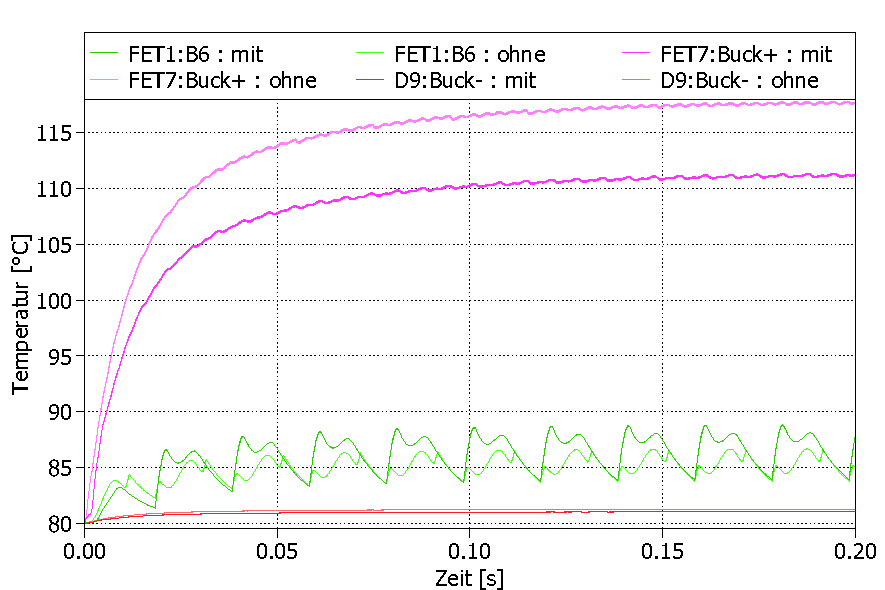
\includegraphics[width=0.9\linewidth]{content/Grafiken/B6_Temp_0&30Grad}
		\caption{Temperaturverhalten der Halbleiter des B6 mit (voll dargestellt) und ohne (schwach dargestellt) Phasenverschiebung}
		\label{fig:b6temp030grad}
	\end{figure}
	Die Eingangsströme sind nur leicht durch die Schaltimpulse verrauscht und der Sinusverlauf folgt wie gewünscht der Eingangsspannung, siehe Abb. \ref{fig:b6acdc0grad}. Es zeigt sich das der Stromverlauf eine \gls{THD} von nur etwa 5,8 \% besitzt. 
	
	\begin{figure}[H]
		\centering
		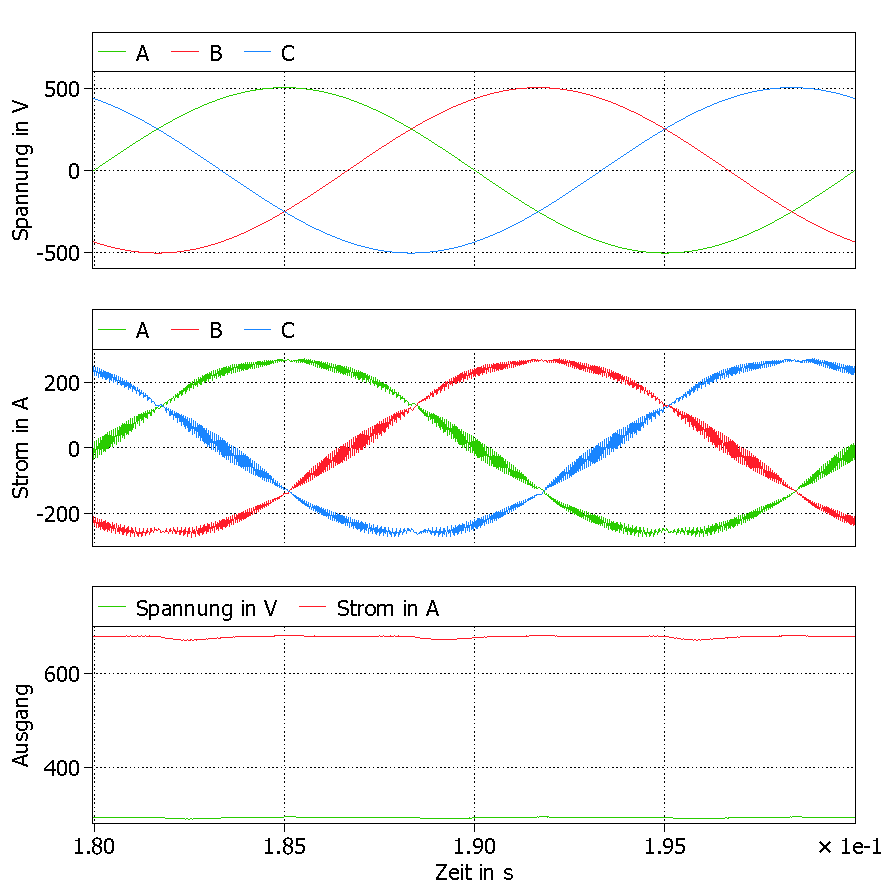
\includegraphics[width=0.9\linewidth]{content/Grafiken/B6_AC+DC_0Grad}
		\caption{Eingangs- und Ausgangsgrößen ohne Phasenverschiebung}
		\label{fig:b6acdc0grad}
	\end{figure}
	Mit Phasenverschiebung von 30 Grad sieht das verhalten ähnlich aus, siehe Abb. \ref{fig:b6acdc30grad}. Der Stromverlauf zeigt eine geringfügig schlechtere THD von 7,1 \%, dies kann durch geeignete Filter ausgeglichen werden. 
\begin{figure}
	\centering
	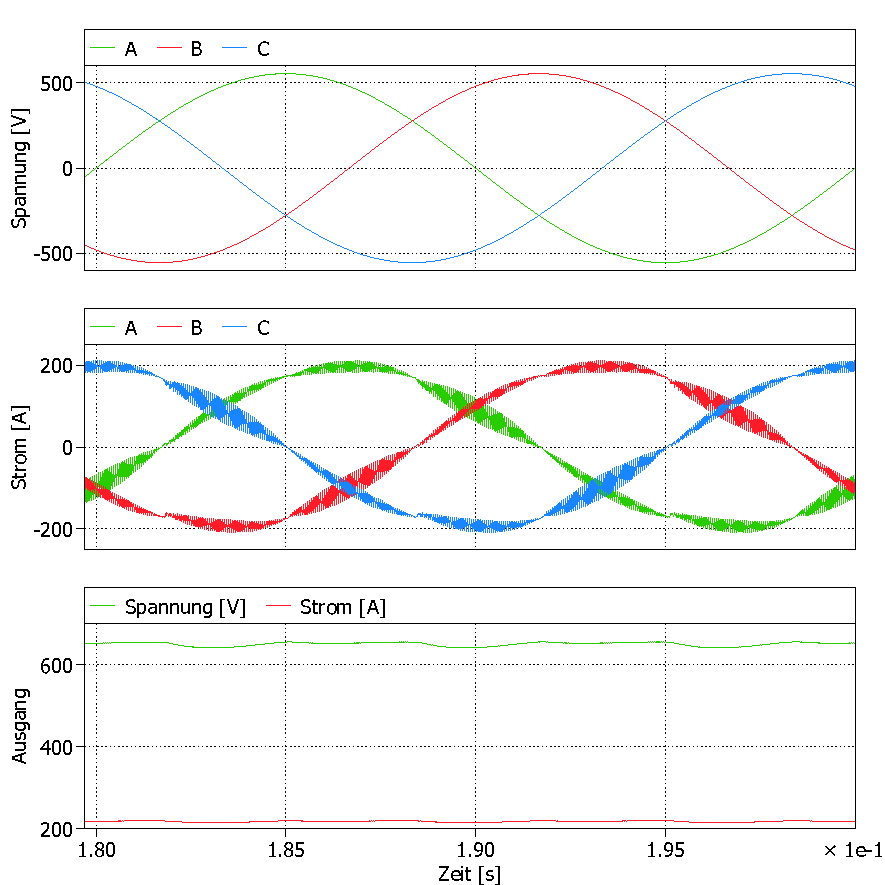
\includegraphics[width=0.7\linewidth]{content/Grafiken/B6_AC+DC_30Grad}
	\caption{Eingangs- und Ausgangsgrößen mit Phasenverschiebung}
	\label{fig:b6acdc30grad}
\end{figure}

\section{IAF}
Für die Auswertung werden die Simulationen für eine Dauer von 0,4 Sekunden laufen gelassen, da dann bereits ein Eingeschwungener Zustand erreicht ist. Das Temperaturverhalten der Halbleiter ist in Abb. \ref{fig:iaftemp} dargestellt, hier kann erkannt werden, dass die Kühlplattentemperatur als Startpunkt den Einschwingvorgang deutlich verkürzt. In grün dargestellt als in (a) höchste Temperatur sind die Dioden des Gleichrichters, da diese den Hauptstrom führen. Die Temperatur dieser liegt bei knapp über 140 °C und ist somit unterhalb der erlaubten maximal Temperatur. In Pink dargestellt, ist die Temperatur der T+/- Halbbrücke, diese steigt ebenfalls bei Blindleistungsbereitstellung. In Rot dargestellt und auch unabhängig von der Blindleistung ist die Temperatur des Tiefsetzstellers.  
\begin{figure}
	\centering
	\subfloat[][]{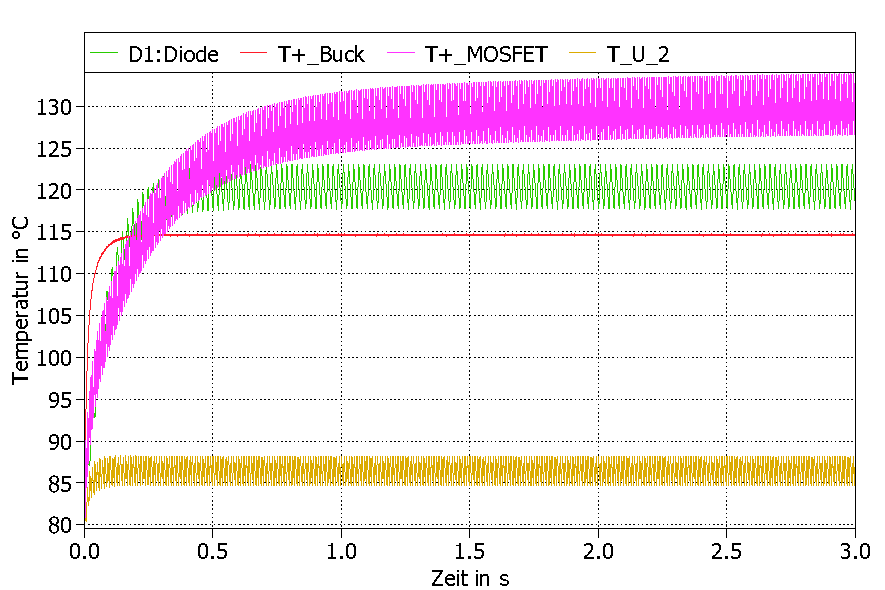
\includegraphics[width=1\linewidth]{content/Grafiken/IAF_Temp_0Grad}}
	\qquad
	\subfloat[][]{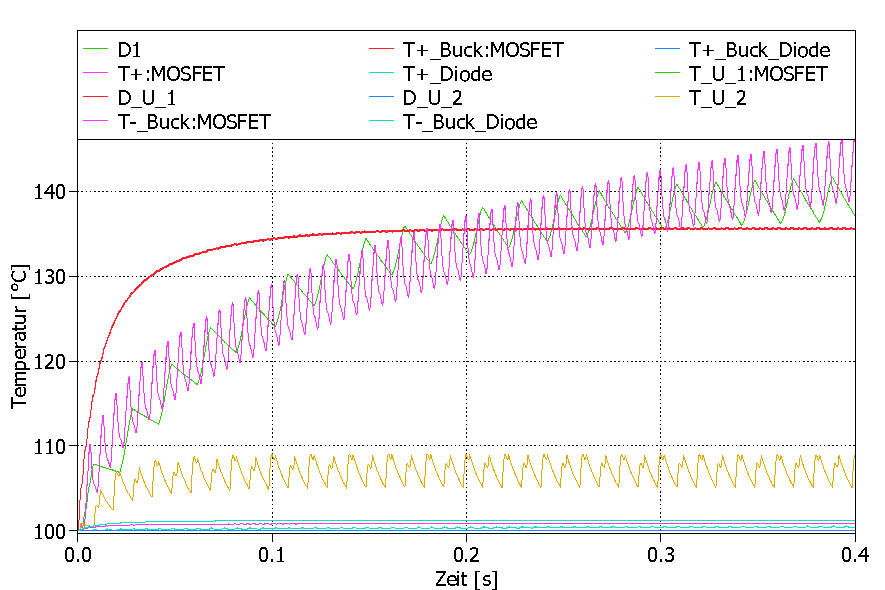
\includegraphics[width=1\linewidth]{content/Grafiken/IAF_Temp_30Grad}}
	\caption{Temperaturverhalten der Halbleiter des IAF ohne (a) und mit (b) Phasenverschiebung}
	\label{fig:iaftemp}
\end{figure}


Die Simulationsergebnisse zeigen den für die Induktivität erwarteten Strom- und Spannungsverlauf mit dreieckiger Form, siehe Abb. \ref{fig:iafacl}. Außerdem ist dem Eingangsstrom ein hochfrequenter Anteil überlagert, welcher sich durch die Schaltfrequenz des Tiefsetzstellers erklären lässt. Außerdem sieht man im Umschaltvorgang des \gls{IVS} starke Sprünge im Stromverlauf, da der Strom in der Induktivität zwischen den Phasen Kommutieren muss.\\
In Abb. \ref{fig:iafacl30grad} zeigt sich dieses Problem aufgrund der starken Spannungsunterschiede zwischen den Phasen bei Phasenverschiebung deutlich stärker. Außerdem muss der \gls{IVS} mehr Strom führen und erzeugt daher stärkere Verlustleistung. Dies ist ebenfalls an der Temperatur des in Abb. \ref{fig:iaftemp} Verlaufs zu erkennen. In (a) ist die Temperatur des IVS in grün dargestellt bei unter 110 °C und in (b) aufgrund des durch die Phasenverschiebung höheren Stroms deutlich gestiegen, bleibt aber unterhalb der zulässigen 175° für die Sperrschichttemperatur..
\begin{figure}
	\centering
	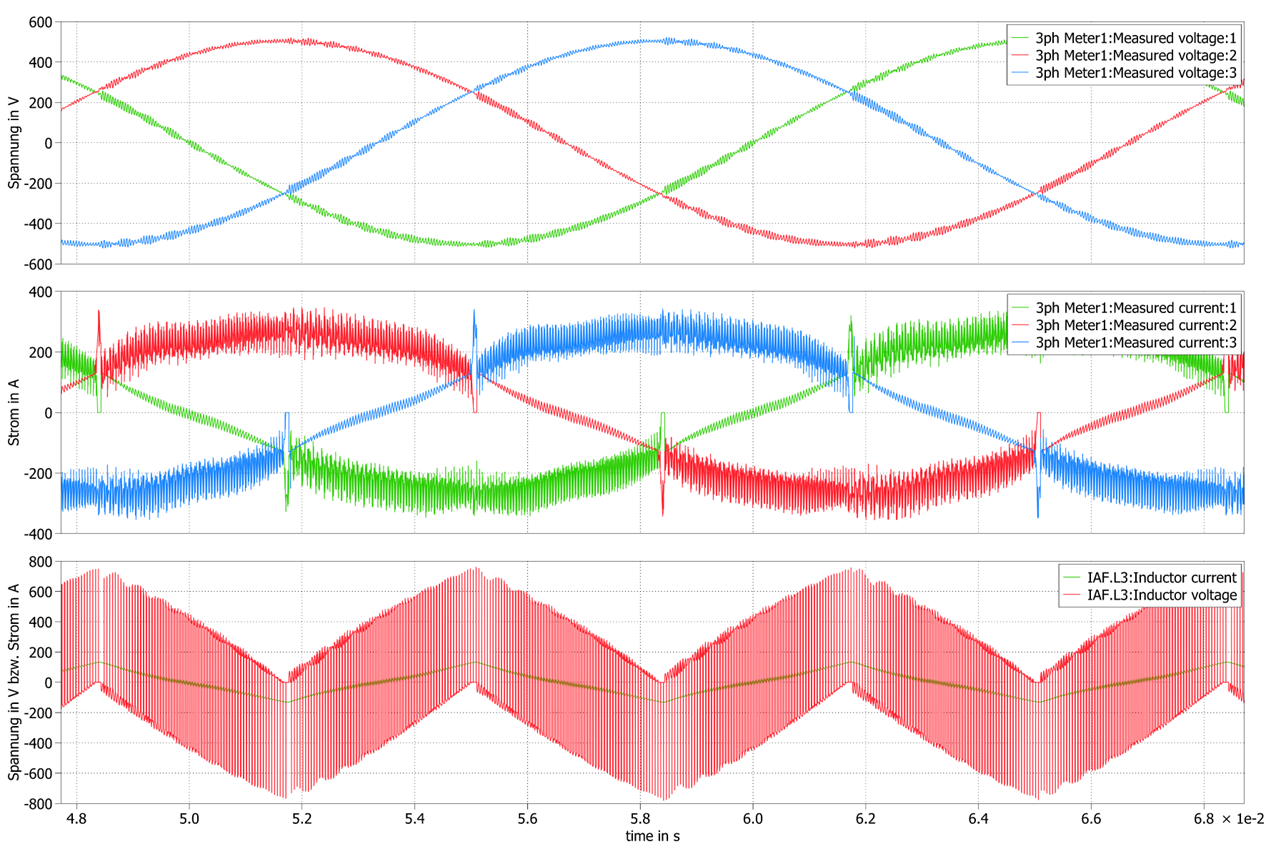
\includegraphics[width=1\linewidth]{content/Grafiken/IAF_AC+L}
	\caption[Simulationsergebnisse des IAF ohne Phasenverschiebung, Eingangsspannung und Ströme, Strom in der IVS Induktivität ]{}
	\label{fig:iafacl}
\end{figure}

\begin{figure}
	\centering
	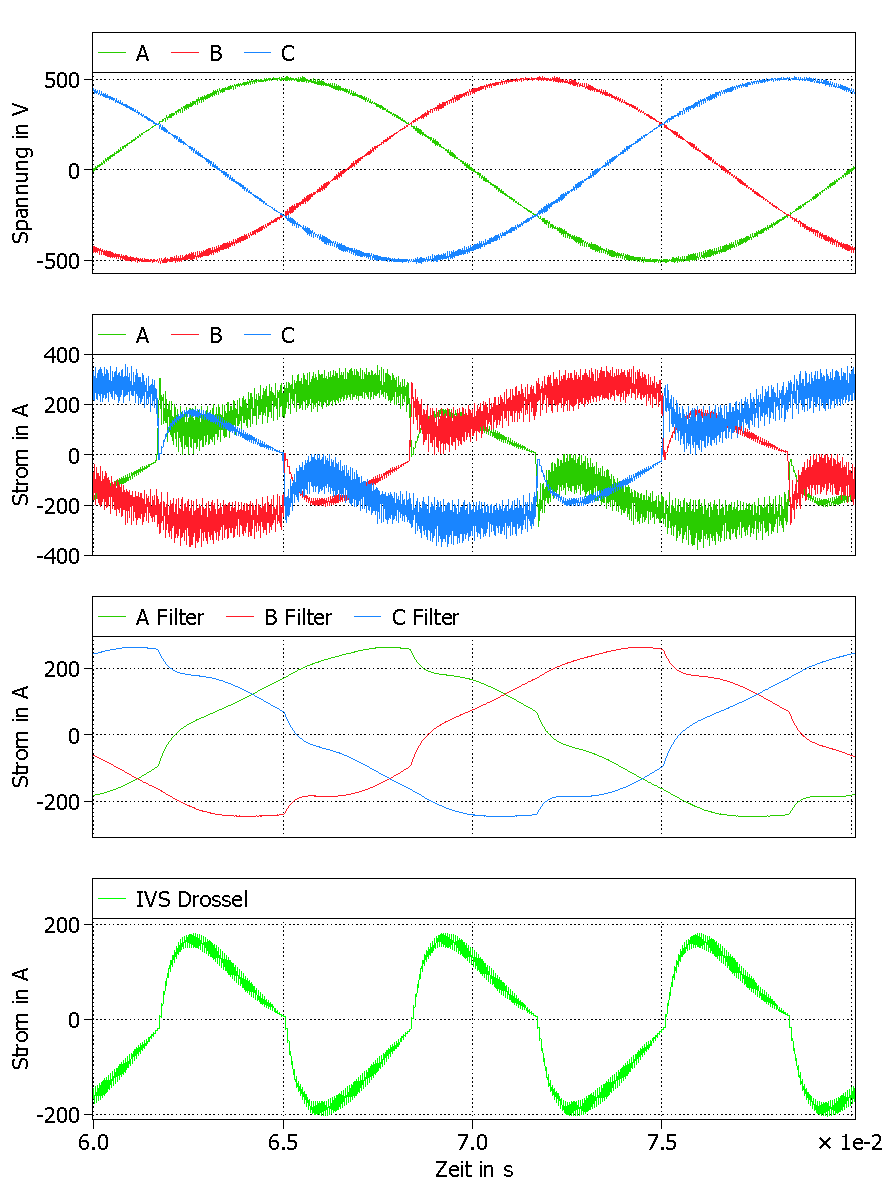
\includegraphics[width=1\linewidth]{content/Grafiken/IAF_AC+L_30Grad}
	\caption{Simulationsergebnisse des IAF bei 30 Grad Phasenverschiebung, Eingangsspannung und Ströme, Strom in der IVS Induktivität }
	\label{fig:iafacl30grad}
\end{figure}
Aufgrund der Anforderung an Blindleistungsbereitstellung hat die Topologie durch den \gls{IVS} einen Nachteil, da dieser sprunghafte Änderungen des Stromverlaufs verursacht. Diese starken Sprünge führen dazu, dass die \gls{THD} des Stroms deutlich verschlechtert wird. Somit kann der \gls{IAF} den Anforderungen nur sehr schwer gerecht werden, da weitere Filterstufen benötigt würden.